\section{System, Assumptions and Problem Formulation}
\label{sec:problemformulation}

\begin{table}[t]
\centering % centering table 
\begin{tabular}{|l|c|c|c|c|c|c|c|} % 
\hline %\hline % inserting double-line 
 & San Francisco & Seattle & Houston & Austin & Dallas \\
\hline %\hline % inserting double-line 
Channels & 2 & 7 & 3 & 1& 3 \\
\hline %\hline % inserting double-line 
\end{tabular}
\caption{Number of White Space Channels in Major Cities} % title name of the table 
\label{tab:whitespacechannel}
\vspace{-0.3in}
\end{table}

% Background and problem model
\subsection{System and Assumptions}
\label{subsec:model}
% Background
% Multiband variation
Wireless propagation refers to the signal loss characteristics when wireless signals 
are transmitted through the wireless medium. The strength of the received signal depends on 
both the line-of-sight path (or lack thereof) and multiple other paths that result from reflection, 
diffraction, and scattering from obstacles~\cite{andersen1995propagation}. The widely-used Friis
equation characterizes the received signal power $P_r$ in terms of transmit power $P_t$, transmitter 
gain $G_t$, receiver gain $G_r$, wavelength $\lambda$ of the carrier frequency, distance $R$ from 
transmitter to receiver, and path loss exponent $n$ according to~\cite{friis}:
\begin{equation}
\label{eq:friis}
P_r=P_t+G_t+G_r+10n \log_{10}\left( \frac{\lambda}{4\pi R}\right)
\end{equation}
Here, $n$ varies according to the aforementioned environmental 
factors with a value ranging from two to five in typical outdoor 
settings~\cite{rappaport}.
% White spcae is good out resource to improve the service of Wifi cell
The propagation range of low-frequency white space channels is many times larger than high-frequency WiFi channels. For instance, 
450 MHz has more than 12 times the propagation range of 5 GHz according to the Friis model. Thus, a 
single white space access point can cover an area up to hundred times of a WiFi access point (if the network was not capacity constrained). 
The large propagation of white space channels can potentially be applied for the reduction of network deployment 
costs~\cite{pcuiwinmee}, adaptation of vehicular dynamic access~\cite{chen2011feasibility}, or improvement 
of network capacity via additional channel resources~\cite{bahl2009white}.
However, previous works that focus on the application of many white space channel resources or point-to-point 
communication requiring a small amount of white space resources often fail to investigate the joint use of WiFi and white space bands with their respective advantages and disadvantages.

% Power saving
\begin{figure}
\vspace{-0.0in}
\centering
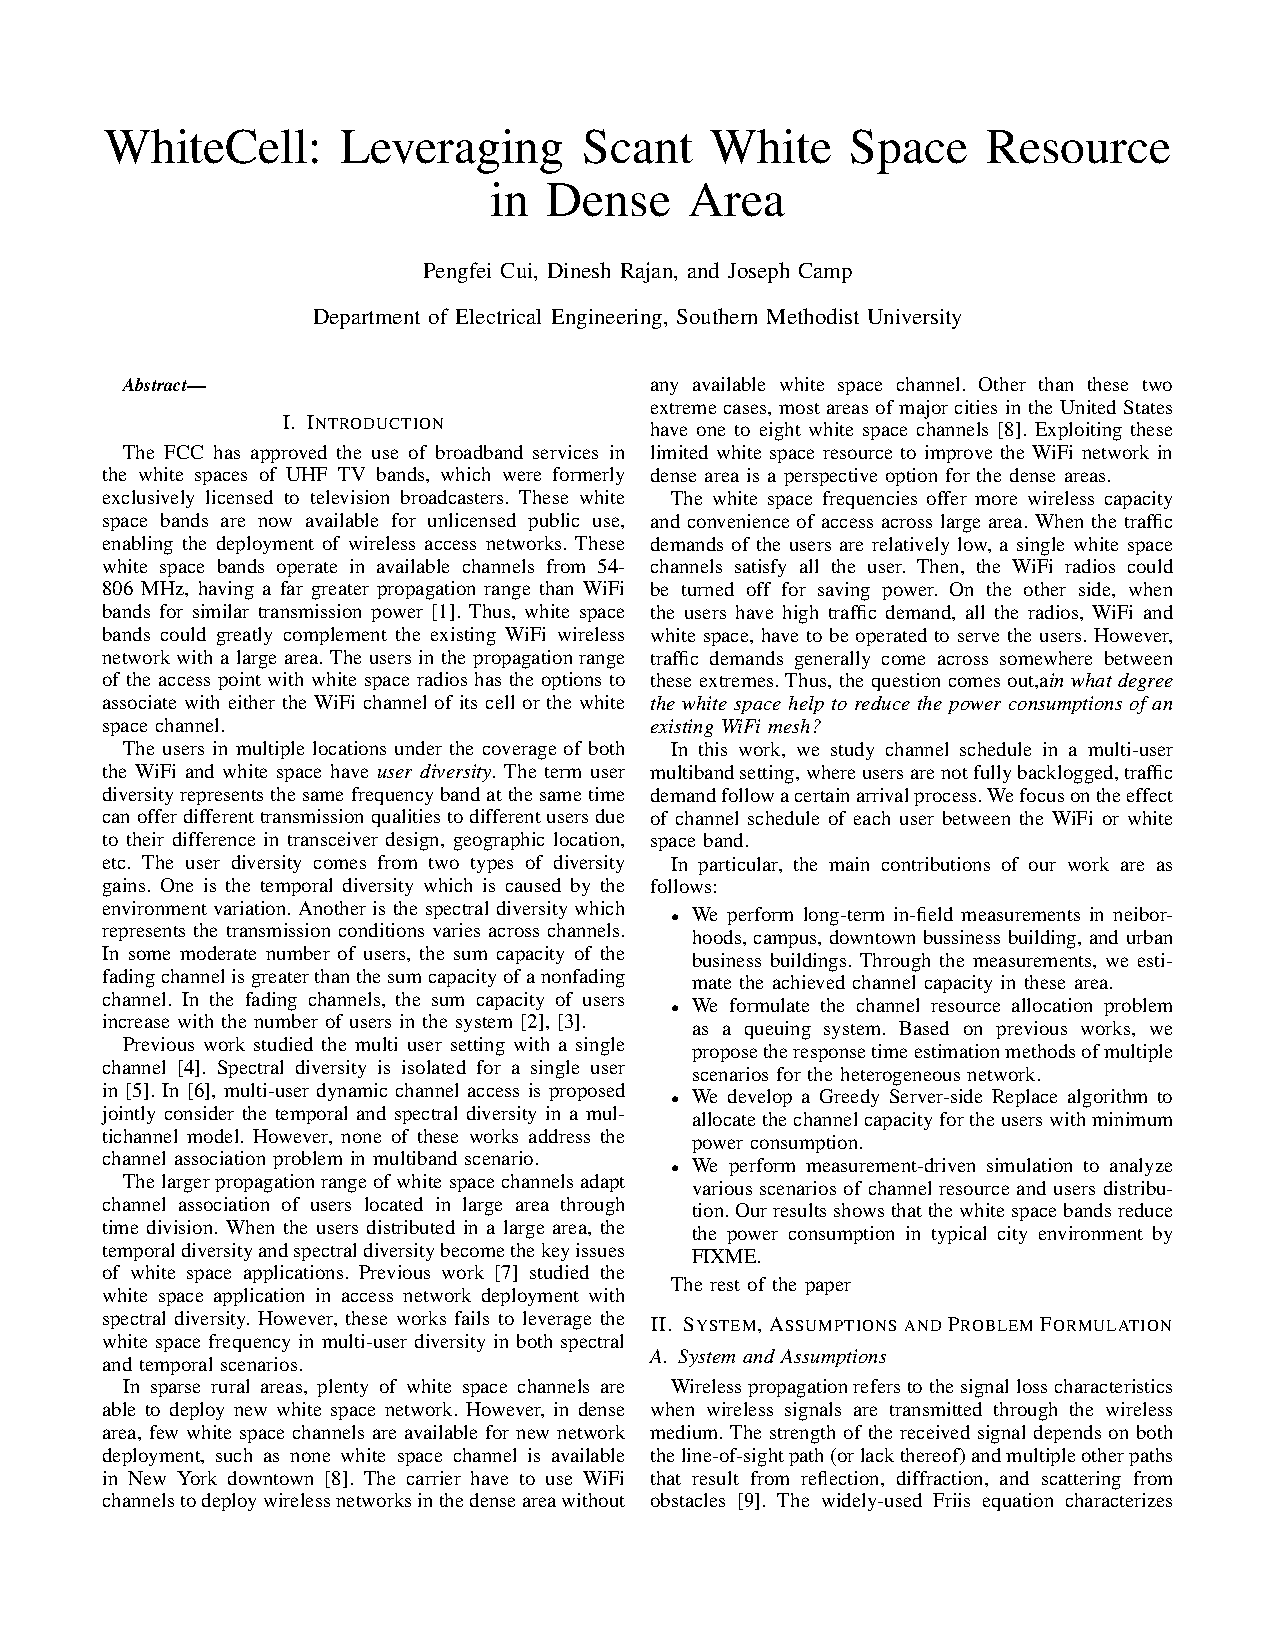
\includegraphics[width=84mm]{figures/whitecell}
\vspace{-0.1in}
\caption{WhiteCell Structure}
\label{fig:systemmodel}
\vspace{-0.3in}
\end{figure}

In wireless network design, a wider range of carrier frequencies allows greater 
flexibility and potentially better performance.  White space frequency bands are a relatively
new opportunity for wireless data networks which have yet to be fully deployed and exploited.
However, the FCC restricts the number of white space channels in most dense urban areas 
to protect existing television broadcasts. 
The minimum number of white space channels in some major cities of the U.S are listed in 
Table~\ref{tab:whitespacechannel}~\cite{googlespectrum}.
In New York and Los Angeles (not listed), some districts have zero white space channel available.
Part of Austin has only one white space channel available in dense urban areas.
Most of the other cities in the table have 2 to 7 white space channels.
Thus, it is infeasible to implement white space wireless networks 
with limited resources in these dense urban areas.
% WiFi cells exist
Moreover, most of the dense areas already have deployed wireless networks. 
Our proposed wireless system leverages the existing infrastructure, adding additional
frequency efficiency and lower energy usage.

% Give the model and assumption
% B channel; N user; M AP;
Here, we introduce a wireless network structure named WhiteCell that leverages an existing
cell site but additionally uses WiFi and white space radios. We assume that each cell contains 
a cellular and WiFi transmitter. However, due to the range of white space transmitters, we 
assume that the central cell can cover all six surrounding adjacent cells with at least
one white space transmitter (as shown in Fig.~\ref{fig:systemmodel}), forming a WhiteCell. 
We assume that these seven smaller cells that compose one WhiteCell can operate independently
of surrounding WhiteCells due to spatial reuse. For our analysis, we will consider up to 
three white space transmitters and channels are available per WhiteCell.
The $N$ users that exist in the WhiteCell network architecture has $M$ access points 
equipped with WiFi and cellular capabilities and $M/7$ cells equipped white space capabilities. 
%The reuse of WiFi and cellular channels has been discussed in plenty of previous works and it is 
%out of our scope.
$F_w$ is the number of white space radios installed on the central cell's access point.
The white space channels are able to be split for multiple cells access point in the system.
We assume the capacity in an environment of each the radios is $C$ if the channel is free
of spectral activity and reduced according to the percentage of time the channel is in use. 
We assume that sufficient memory space exists to buffer traffic to the users from each access point.
The traffic aggregated at the access point could be transferred through the single cell 
frequency resources or the shared white space resources.
The traffic is served in a first-in-first-out (FIFO) scheduling strategy.
In this structure, the traffic of each cell could be transferred by $F_w+1$ channels.
The one is the single cell wireless channel and the others are the white space channels.
We assume the users in the same mesh cell are in a single interference domain. 
Considering the limited number of white space channels in dense areas and considering spatial reuse 
of white space makes the problem considerably more challenging, it remains an interesting 
direction for future research. 

Instead of assuming the wireless channels are on-off~\cite{bodas2012low} or have equal capacity, 
we apply a measurement driven estimation to get the achieved channel capacity. The capacity of the 
channel between the access points and each user is noted as a matrix in Eq.~\ref{eq:usercapacity}
\begin{equation}
\label{eq:usercapacity}
H_{i,j}^f(t)= G(\zeta,t),i \in M, j\in N, f \in (F_M+F_w) 
\end{equation} 
$\zeta$ represents the in-field measured historical data and dynamic sensing information.
A context-aware method is applied to estimate the $j$th user capacity $H_{i,j}^f(t)$ to an access point 
$i$ on channel $f$. The users in a single cell have the same channel status. We assume the channel 
capacity is flat during a certain time slot. The switching time is negligible in the system.
The calculation of achieved channel capacity is introduced in~\ref{subsec:experimentsetup}. 
The traffic demand of a user obey Poisson process, with the vector noted as 
$\bm{D(t)} = [D_1(t),D_2(t),...D_N(t)]$ and the sum rate $D(t) = \sum\limits_{i=1}^N D_i(t)$. 
The rate $D(t)$ is the aggregate rate of data generated from all users. 

% tolerance time, energy model
During a time slot, the unscheduled radios remain in sleep mode to save energy. We also ignore 
the sleeping energy as well as the amount of energy spent on channel or radio switching. An operating 
radio will cost equal standby power per unit time. Previous human factor work~\cite{niida2010user} 
shows users have a certain patience for response. 
The tolerance time of users varies across the traffic type, such as text information, 
voice and video. To simply the problem, we assume an average value for tolerance response time $W$ 
of all the users in the system. 
With the same number of traffic demand, more channel capacity offers more data rate which reduce 
the response time.
Thus, the longer the tolerance time required by the users, the more channel capacity resource is 
required.

\subsection{Problem Formulation}
\label{subsec:problem}

We formulate the wireless network system introduced in~\ref{subsec:model} as a 
discrete-time queuing system shown in Fig.~\ref{fig:flowconfig}. 
The channels are represented as servers in the queuing model. 
Table.~\ref{tab:notation} summarizes the notation used in this work. 
In the system, there are $F_w$ white space radios and $M$ cells. 
$F_M$ represents the single cell resource radios allocated to $M$ cells. 
Multiple cells may share the same single cell resource, but there is no overlap of their service areas.
Thus, the queuing system has $M$ queues of the cells and $F_M+F_w$ servers in total connecting 
by time-varying channels $H^*(M,F_M+F_w)$.

\begin{table}[htbp]
\begin{center}% used the environment to augment the vertical space
% between the caption and the table
\begin{tabular}{l l p{10cm} }
\toprule
$t$ & Time slot\\
$N$ & Set of users\\
$M$ & Set of WiFi cells\\
$H_{ij}^f$ & Measurement based Capacity between AP i and user j on channel f\\
$F_{m}$ & WiFi Channels in the cells\\
$F_{w}$ & Set of White Space Channels\\
$A(t)$ & User access channel schedule\\
$C$ & Clean Radio Capacity\\
$D$ & User Demand\\
$R$ & Operating Radio\\
$\zeta$ & In-Field Measurements\\
$W$ & User Tolerance time window \\
$\mu$ & Channel capacity assigned for a cell \\
$P_s$ & Standby Power Consumption \\
$P_t$ & Transmission Power Consumption \\
%$R_{i}$ & $\triangleq$ & Revenue at store $i$\\
%$i$ & $\triangleq$ & index value for store locations\\
%${T}_{c}$ & $\triangleq$ & A very long description of this specific variable and is needed in the research and looks good when wrapped and aligned to the left.\\
%$TC$ & $\triangleq$ & Total overall cost(\$)\\  
%\multicolumn{3}{c}{}\\
%\multicolumn{3}{c}{\underline{Decision Variables}}\\
%\multicolumn{3}{c}{}\\
%$y_f$ & $=$ & \(\left\{\begin{array}{rl}
%1,  & \text{if Supplier located at site $f$ is open} \\
%0,  & \text{otherwise} \end{array} \right.\)\\
\bottomrule
\end{tabular}
\end{center}
\caption{Table of Notations}
\label{tab:notation}
\vspace{-0.3in}
\end{table}


\begin{figure}
\vspace{-0.0in}
\centering
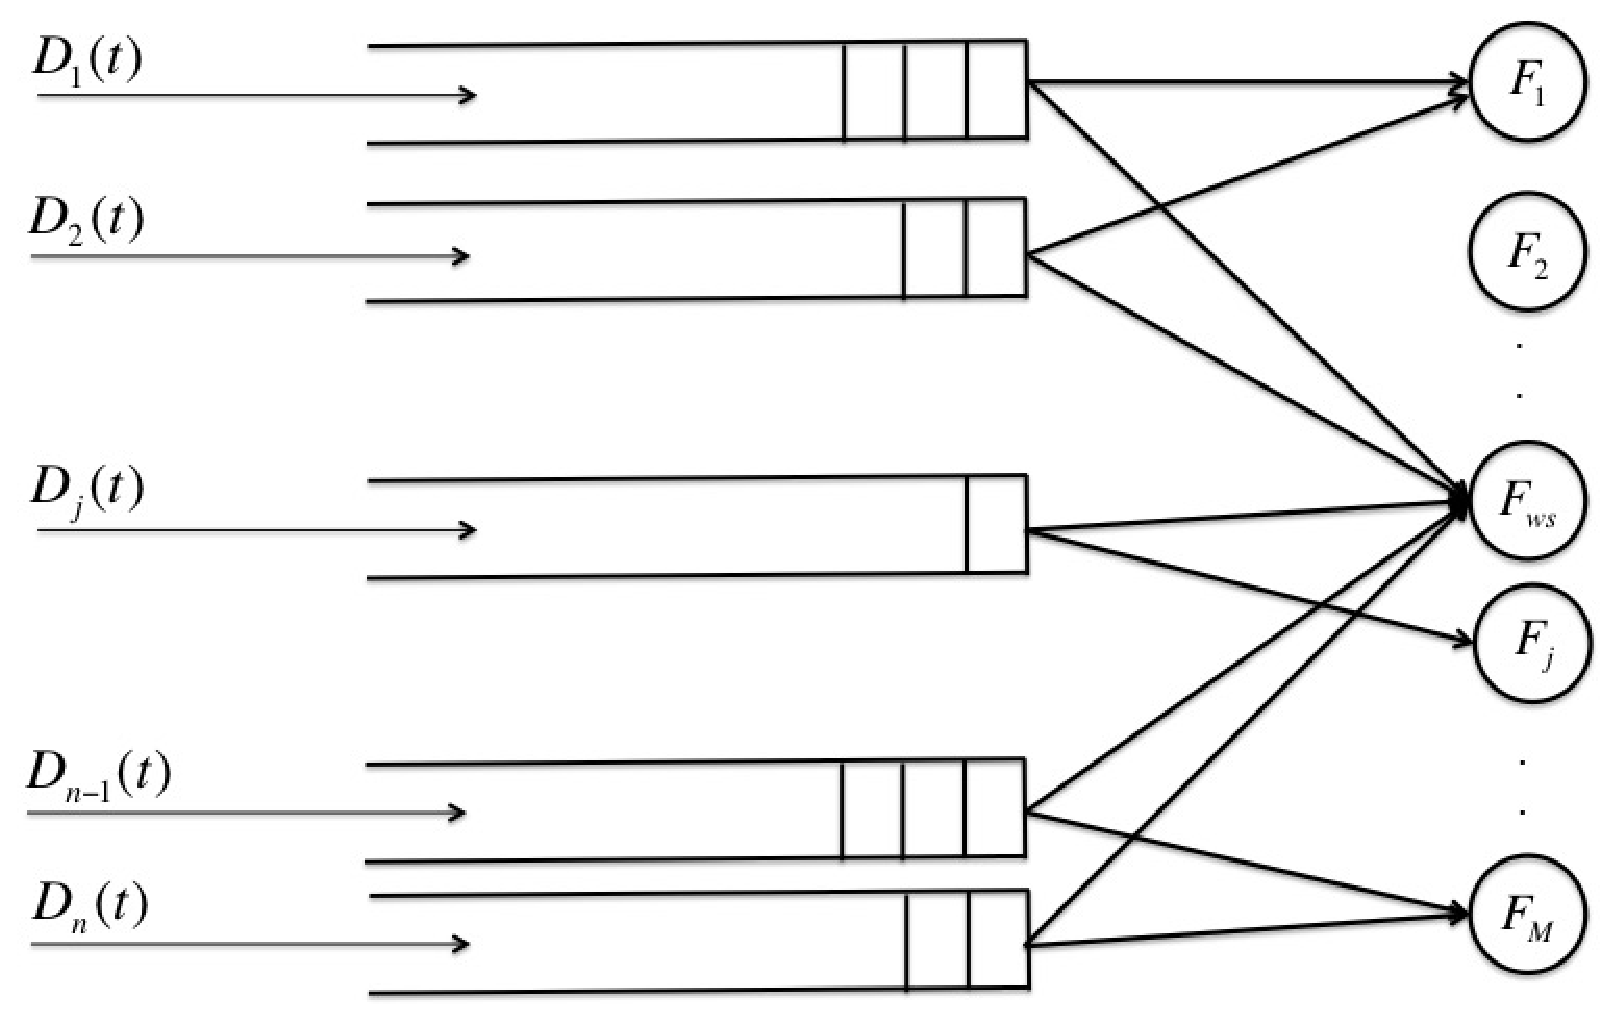
\includegraphics[width=84mm]{figures/flowconfig}
\vspace{-0.1in}
\caption{System Model}
\label{fig:flowconfig}
\vspace{-0.3in}
\end{figure}

The matrix \{$A_{i,j}(t),i\in (F_M+F_w), j\in M$\} denotes the wireless resource association
as shown in Eq.~\ref{eq:associate_def}.
%where $A_{i,j}^b = 1$ denotes user $j$ is scheduled with access point $i$ on channel $b$.
\begin{equation}
\label{eq:associate_def}
 A_{i,j}(t) = \left\{ 
	  \begin{array}{l l}
	    1   &  if\ D_{j\in M},\ is\ associated\ with\ \\
		& radio\ i \in (F_M+F_w) \\
		0 &  Otherwise
			    \end{array} \right.
\end{equation}

To keep the quality of service, the queuing system restricts the expected response time of 
the system $w$ to no more than the tolerance threshold $W$ as shown in Eq.~\ref{eq:timeconstraint}
\begin{equation}
\label{eq:timeconstraint}
E[w]\le W
\end{equation}

% Extreme examples
When the total traffic demand of the users in the system are relatively small, 
the channel capacity of a single white space channel could achieve the quality of 
service in response time for all the users. 
In this scenario, all cell radios could be switched to sleep mode for power saving. 
On the other hand, as the traffic demand increase with the number of users or the demand per 
user, the channel resources need to be increased as the number servers in the queuing system increment 
to meet the user response time tolerance requirements. Thus, in this extreme case, all the radios 
have to keep operating to provide the appropriate quality of service. 
Moreover, when the users are distributed non-uniformly, the long propagated white space channels 
are able to deliver more capacity for the cells with more traffic to balance the system load 
without adding new infrastructure. 
The flexibility of white space channels offers new opportunity for power saving and 
offer load adaptation in network design.
To apply these white space advantages, the question {\it can we save power by exploiting 
the white space capacity with existing cells?} has to be addressed in this system.

In this work, we focus on analyzing the power savings for the  
WhiteCell system. 
To model the power consumption of the system, we sum the power consumption of each operating 
radio in two power consumption categories: standby and transmitting.
We assume the sleeping standby power consumption is negligible as well as the switching power consumption. 
We define $R_i$ represents the radios status in the system, $i\in {F_w,F_M}$. 
The value of $R_i$ denotes the power consumption of the radio for standby and transmitting.
When the radio is in sleeping mode, $R_i = 0$. 
The definition is as represented in Eq.~\ref{eq:radio}.

\begin{equation}
\label{eq:radio}
 R_i(t) = \left\{ 
	  \begin{array}{l l}
	    P_s+P_t\cdot\mu   &  \sum\limits_{j=1}^N A_{i,j}(t) \ge 1\\
		0 &  Otherwise
			    \end{array} \right.
\end{equation}

% Explain the equation
$P_s$ is the standby power consumption of a radio which is a constant value, $P_t$ is the 
unit transmit power consumption of the assigned channel capacity. 
$\mu$ is the allocated channel capacity of the radio.
$R_i(t)$ is the power consumption of the radio during the time slot.

Thus, to reduce the power consumption of the system, it could be 
implemented via minimizing the sum of $R_i$ under the quality of service constraints. 
The objective is to minimize the power consumption of the system is represented in Eq.~\ref{eq:objective}:
\begin{equation}
\label{eq:objective}
R^*(t) = \min{\{\sum\limits_{i=1}^{(F_M+F_w)} R_{i}}(t)\}
%\xi = \min{\{\sum\limits_{t}^{t+T}\sum\limits_{i}^{(F_M+F_w)} R_{i}}(t)\}
\end{equation}
$R^*$ represent the minimum operating power consumption required of the system. 
The allocated resources $\mu$ could be adjusted to approach the minimum power consumption 
in the model. 
According to the queuing quality of service model and power consumption model, 
we further analyze the WhiteCell system and propose our greedy solution.

